\documentclass{article}
\usepackage[utf8]{inputenc}
\usepackage{graphicx}
\usepackage[margin=1in]{geometry}
\usepackage[dvipsnames]{xcolor}
\usepackage{url}
\usepackage{hyperref}
\usepackage[numbers]{natbib} % for numeric references

\begin{document}

\begin{titlepage}
    \begin{center}
        \textbf{\LARGE Does Money Buy a Longer Life?}\\
        \textbf{\LARGE The Preston curve for 158 countries in 2019}

        \vspace{1.5cm}

        \textbf{\Large Szymon Stembalski (i6389327)}

        \vspace{1cm}

        \IfFileExists{figures/MSP-logo.jpg}{
\includegraphics[width=3cm]{figures/MSP-logo.jpg}}{}

        \vfill

        \large Date: \today

    \end{center}
\end{titlepage}

\newpage

\section*{Introduction}
People in rich countries live much longer than people in poor countries. In
2019 a child born in Japan could expect to live 85 years, while a child born in
Nigeria could expect 63. In 1975 the demographer Samuel Preston showed that
life expectancy rises steeply with income in poor countries and levels off in
rich ones~\cite{preston}. This relation is now called the \emph{Preston curve}.
It matters for policy: if extra income buys many years of life in poor
countries but only a few in rich ones, then economic growth is most valuable
for health where people are poorest.

In this report we ask: \textbf{how many years of life expectancy go together
with a doubling of a country's income? And is this gain smaller for rich
countries than for poor ones?}

\section*{Data sample}
We use the Gapminder ``Fast Track'' dataset~\cite{gapminder}. It is a
collection of CSV files with one value per country per year, compiled by
Gapminder from the UN, the World Bank and other sources. We use three
variables:
\begin{itemize}
  \item \texttt{lex}: life expectancy at birth, in years;
  \item \texttt{gdp\_pcap}: GDP per capita in international dollars, adjusted
        for inflation and for purchasing power (PPP), so that incomes can be
        compared between countries;
  \item \texttt{pop}: population, used to drop very small countries.
\end{itemize}
We also use the country names and the world region of each country.

We use the year 2019, the last year before the COVID-19 pandemic, which
temporarily lowered life expectancy in many countries. We drop countries with
fewer than one million inhabitants, because their data are noisier. No further
cleaning is needed: all three variables are available for every remaining
country. The final sample has \textbf{158 countries}. Life expectancy ranges
from 53.8 to 85.4 years, and GDP per capita ranges from \$583 to \$120\,114.

\section*{Data analysis method}
The analysis is a single Python script using \texttt{pandas},
\texttt{scipy} and \texttt{matplotlib}. Plotted against income, life
expectancy rises quickly at first and then levels off. Plotted against the
\emph{logarithm} of income, the relation is close to a straight line
(Figure~\ref{fig:preston}). We therefore fit
\begin{equation}
  \mbox{life expectancy} = a + b \cdot \log_2(\mbox{GDP per capita})
\end{equation}
by least squares, with each country counted once. Using $\log_2$ makes the
slope $b$ easy to read: it is the number of years of life expectancy that go
together with a \emph{doubling} of income. The uncertainty on $b$ is the
standard error from the fit.

To test whether the gain gets smaller for rich countries, we split the sample
at the median GDP per capita (\$15\,053) and fit each half separately. We then
compare the two slopes. The uncertainty on their difference is
$\sigma_{\Delta b} = \sqrt{\sigma_{\rm poor}^2 + \sigma_{\rm rich}^2}$.

\section*{Results and discussion}

\begin{figure}[h]
  \centering
  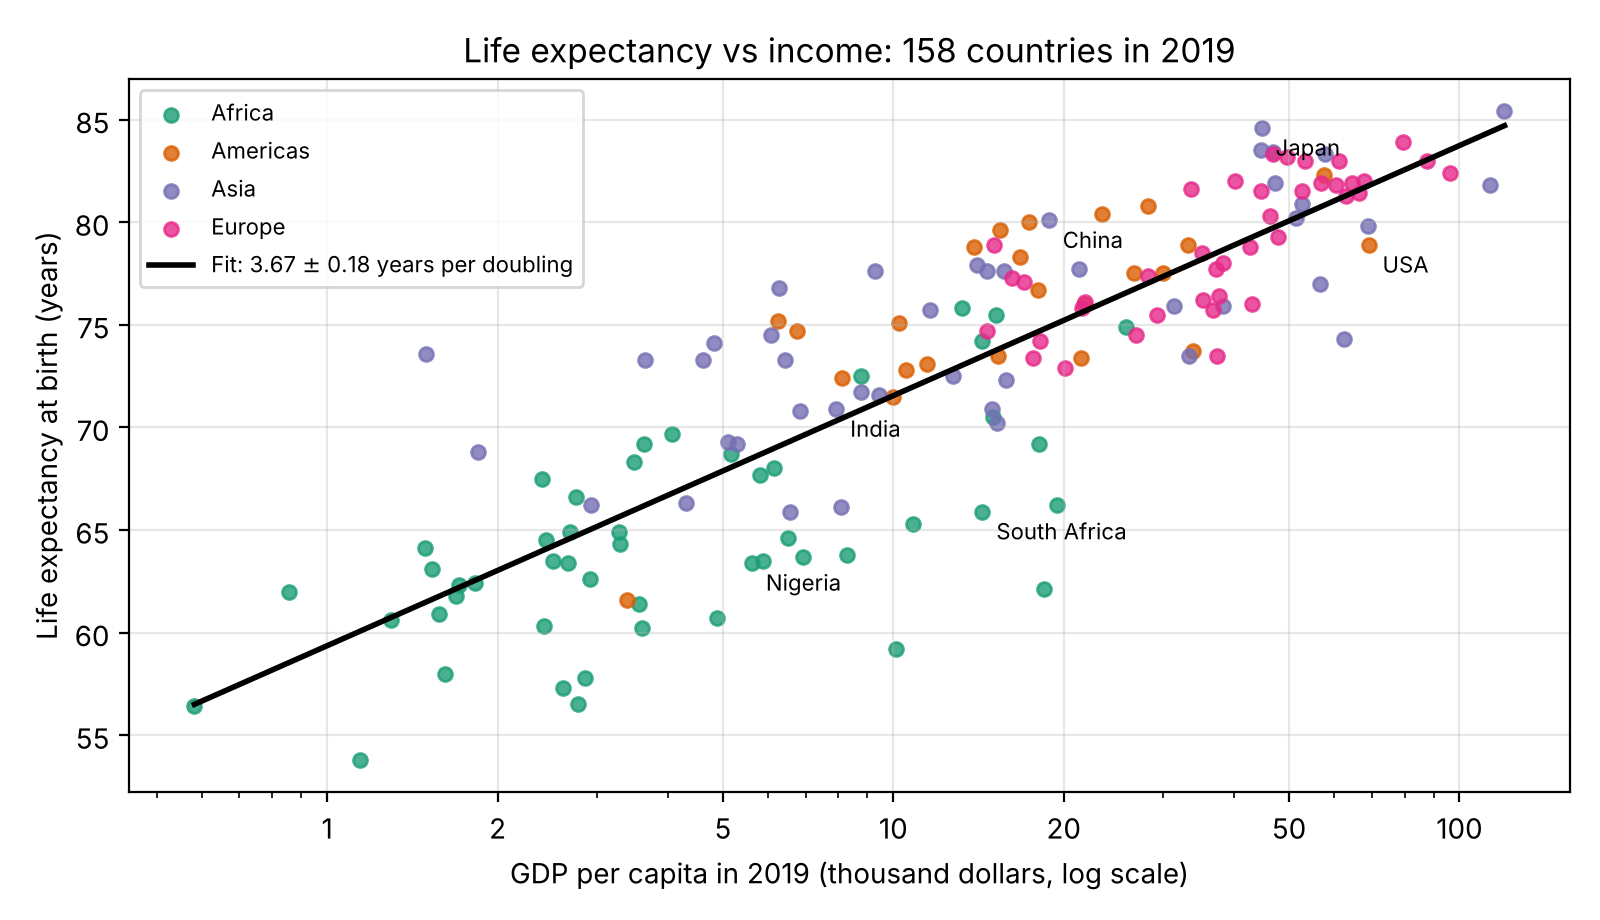
\includegraphics[width=0.85\linewidth]{figures/preston_curve.png}
  \caption{Life expectancy against GDP per capita for 158 countries in 2019.
  Each dot is a country, coloured by world region. The income axis is
  logarithmic. The black line is the fit of Eq.~(1).}
  \label{fig:preston}
\end{figure}

The fit gives
\[
  b = 3.67 \pm 0.18 \ \mbox{years per doubling of income}, \qquad
  a = 22.8 \pm 2.5 \ \mbox{years}.
\]
The correlation is strong: $r = 0.85$, so income alone explains
$R^2 = 73\%$ of the differences in life expectancy between countries.
The scatter of countries around the line is 3.9 years.

For the poorer half of the countries we find
$b_{\rm poor} = 3.64 \pm 0.45$ years per doubling, and for the richer half
$b_{\rm rich} = 3.46 \pm 0.47$ years per doubling. The difference is
$0.18 \pm 0.66$ years, only $0.3\sigma$. The two halves are therefore
consistent with one and the same slope. In other words, the gain does
\emph{not} get smaller per doubling of income.

The curve still flattens in absolute terms, because a doubling costs very
different amounts of money. Going from \$1\,000 to \$2\,000 per person and
going from \$50\,000 to \$100\,000 both add about 3.7 years. The first needs
\$1\,000 extra, but the second needs \$50\,000. So an extra \$1\,000 goes
together with about 50 times more years of life in a poor country than in a
rich one.

Income does not explain everything. China (+5.2 years) and Japan (+5.1)
live longer than their income predicts, and the USA lives 2.9 years shorter.
The largest negative deviations are in southern Africa, for example Eswatini
($-12.4$ years) and South Africa ($-7.6$), where HIV/AIDS strongly lowers
life expectancy. They are also found in oil-rich countries such as Equatorial
Guinea ($-12.7$), whose high GDP per capita is not shared widely.

\textbf{Conclusion.} Each doubling of income goes together with
$3.67 \pm 0.18$ more years of life expectancy. The slope is the same for poor
and rich countries within $0.3\sigma$. In dollars, however, the gain is far
larger for poor countries, which supports Preston's original finding. Note
that this is a correlation, not proof that money causes longer lives: richer
countries also have better health care, education and sanitation.

\noindent\textbf{Use of AI tools.} I used Claude to help write and debug the Python code, and to draft the README and report. I chose the research question, ran the analysis on my own laptop, checked the results, and can explain all steps of the method and the code.

\begin{thebibliography}{9}
\bibitem{preston}
S.~H.~Preston, \textit{The changing relation between mortality and level of
economic development}, Population Studies \textbf{29}(2), 231--248 (1975).

\bibitem{gapminder}
Gapminder Foundation, \textit{Gapminder Fast Track dataset}. Available at:
\url{https://github.com/open-numbers/ddf--gapminder--fasttrack}
(commit \texttt{85af9e1}, accessed October 2026).
\end{thebibliography}

\end{document}
